\section{Algorithm Description}
\subsection{Genetic Algorithm}
\label{ssec:GenAlg}
The algorithm must determine positions and number of luminaries in dependency on target illuminance and uniformity. This is the multicriteria and multiparametric type of the problem. The genetic algorithms offer quite simple way how to solve it, therefore they were used in this project. The genetic algorithms are well known today so only specific settings are further described.

The best solution was saved (elitism) from every population in two specimens. The first one was unable to change its DNA via mutation, the second one had the same probability of mutation like other solutions. Other parent solutions were selected via tournament selection. It consisted of making random group of $4$ solutions from the population and take the one with the best fitness. This type of selection had vital role in the algorithm. It avoided a premature convergence of the best solution in comparison with the roulette selection. Similar effect was ensured also by setting the recombination probability less than $1$. There was used only one point DNA crossover during presented tests. Overview of the GA settings is shown in Tab.~\ref{tab:GAsettings}.

\begin{table}[htb]
	\renewcommand{\arraystretch}{1.3}
	\caption{Genetic Algorithm Settings}
 	\label{tab:GAsettings}
	\centering
  \begin{tabular}{| l | c |}
    \hline
    \textbf{First Population} & Random logic vectors \\
    \hline
    \textbf{Termination Cond.} & Maximum number of generations \\
    \hline
		\textbf{Number of Gen.} & $30$ \\
    \hline
		\textbf{Population Size} & $50$ \\
    \hline
		\textbf{Recombination Prop.} & $90 \%$ \\
    \hline
		\textbf{Mutation Prop.} & $4 \%$ \\
    \hline
		\textbf{Parent Selec.} & Tournament 1 of 4 \\
    \hline
		\textbf{Mutation Mech.} & Inverted bit \\
    \hline
		\textbf{Survival Selec.} & Elitism \\
    \hline
  \end{tabular}
\end{table}

\subsection{Fitness Function}
\label{ssec:FitFn}
The fitness function defines how good the solutions are. The target value of average maintained illuminance and target value of uniformity are watched in the algorithm. In common case the average illuminance is given especially by a count of the luminaires. The uniformity is given especially by specific positions of the luminaires on the other hand. The count of the luminaires is proportional to investment cost of the lighting system. So the number of luminaires that exactly fulfill the target average value of illuminance is appropriate. The uniformity is always required as much as possible for defined number of luminaires. The fitness function was determined within discussed facts as follows:

\begin{equation}
\label{eq:fitness}
f_{DNA}\left(\overline{E}_{m}, U_0\right) = g_1\left(\overline{E}_{m}\right) + g_2\left(U_0\right)
\end{equation}

\begin{subnumcases}{\label{eq:fitnessG1} g_1\left(\overline{E}_{m}\right)=} 
  e^{\frac{\overline{E}_{m}-\overline{E}_{mT}}{\overline{E}_{m}}} &, $\left\langle 0, \overline{E}_{mT}\right\rangle$ \label{eq:fitnessG1A}\\
  e^{\frac{\overline{E}_{mT}-\overline{E}_{m}}{\overline{E}_{m}}} &, $\left( \overline{E}_{mT}, \infty\right)$ \label{eq:fitnessG1B}
\end{subnumcases}

\begin{subnumcases}{\label{eq:fitnessG2} g_2\left(U_0\right)=} 
  \frac{U_0}{2\cdot U_{0T}} &, $\left\langle 0, U_{0T}\right\rangle$ \label{eq:fitnessG2A}\\
  1-\frac{e^{\frac{U_{0T}-U_0}{U_{0T}}}}{2} &, $\left( U_{0T}, \infty\right)$ \label{eq:fitnessG2B}
\end{subnumcases}

where:
\begin{description}
	\item[$\overline{E}_{m}$] is a calculated maintained average value of illuminance,
	\item[$\overline{E}_{mT}$] is a target maintained average value of illuminance,
	\item[$U_0$] is a calculated lighting uniformity,
	\item[$U_{0T}$] is a target lighting uniformity.
\end{description}

The function $g_1\left(\overline{E}_{m}\right)$ has peak value equal to $1$ at the target value of average illuminance. Because the illuminance cannot be less than zero, the function reaches two limits:
\begin{equation}
\label{eq:g1lim0}
\lim_{\overline{E}_{m}\to 0+} g_1\left(\overline{E}_{m}\right) = 0
\end{equation}
\begin{equation}
\label{eq:g1limInf}
\lim_{\overline{E}_{m}\to \infty} g_1\left(\overline{E}_{m}\right) = e^{-1}
\end{equation}

Both limits have different values and the limit in the infinity is higher than that in the $0$. Hence it is preferred the solution with the higher average illuminance for the same absolute difference from the target value.

The function $g_2\left(U_{0}\right)$ reach the value $0.5$ at the target value of uniformity. It has a bound at $0$ for values less then the target value. There is a limit in the infinity for values higher than target value:
\begin{equation}
\label{eq:g2limInf}
\lim_{U_{0}\to \infty} g_2\left(U_{0}\right) = 1
\end{equation}

So the function $g_2\left(U_{0}\right)$ has an horizontal asymptote equal to one. Function $g_2\left(U_{0}\right)$ is linear for values of uniformity less than the target value. The highest slope is obtained here. The slope is  smaller for higher values of uniformity due to the saturation effect of the exponential function. Therefore the algorithm is forced to reach target value of the uniformity because of big change in the fitness function at its beginning. Higher values improves the fitness function too, but there is a smaller effect.

Both functions $g_1\left(\overline{E}_{m}\right)$ and $g_2\left(U_{0}\right)$ are shown in figure~\ref{fig:fitG1G2} for better understanding.

\begin{figure}[htb]
  \centering
  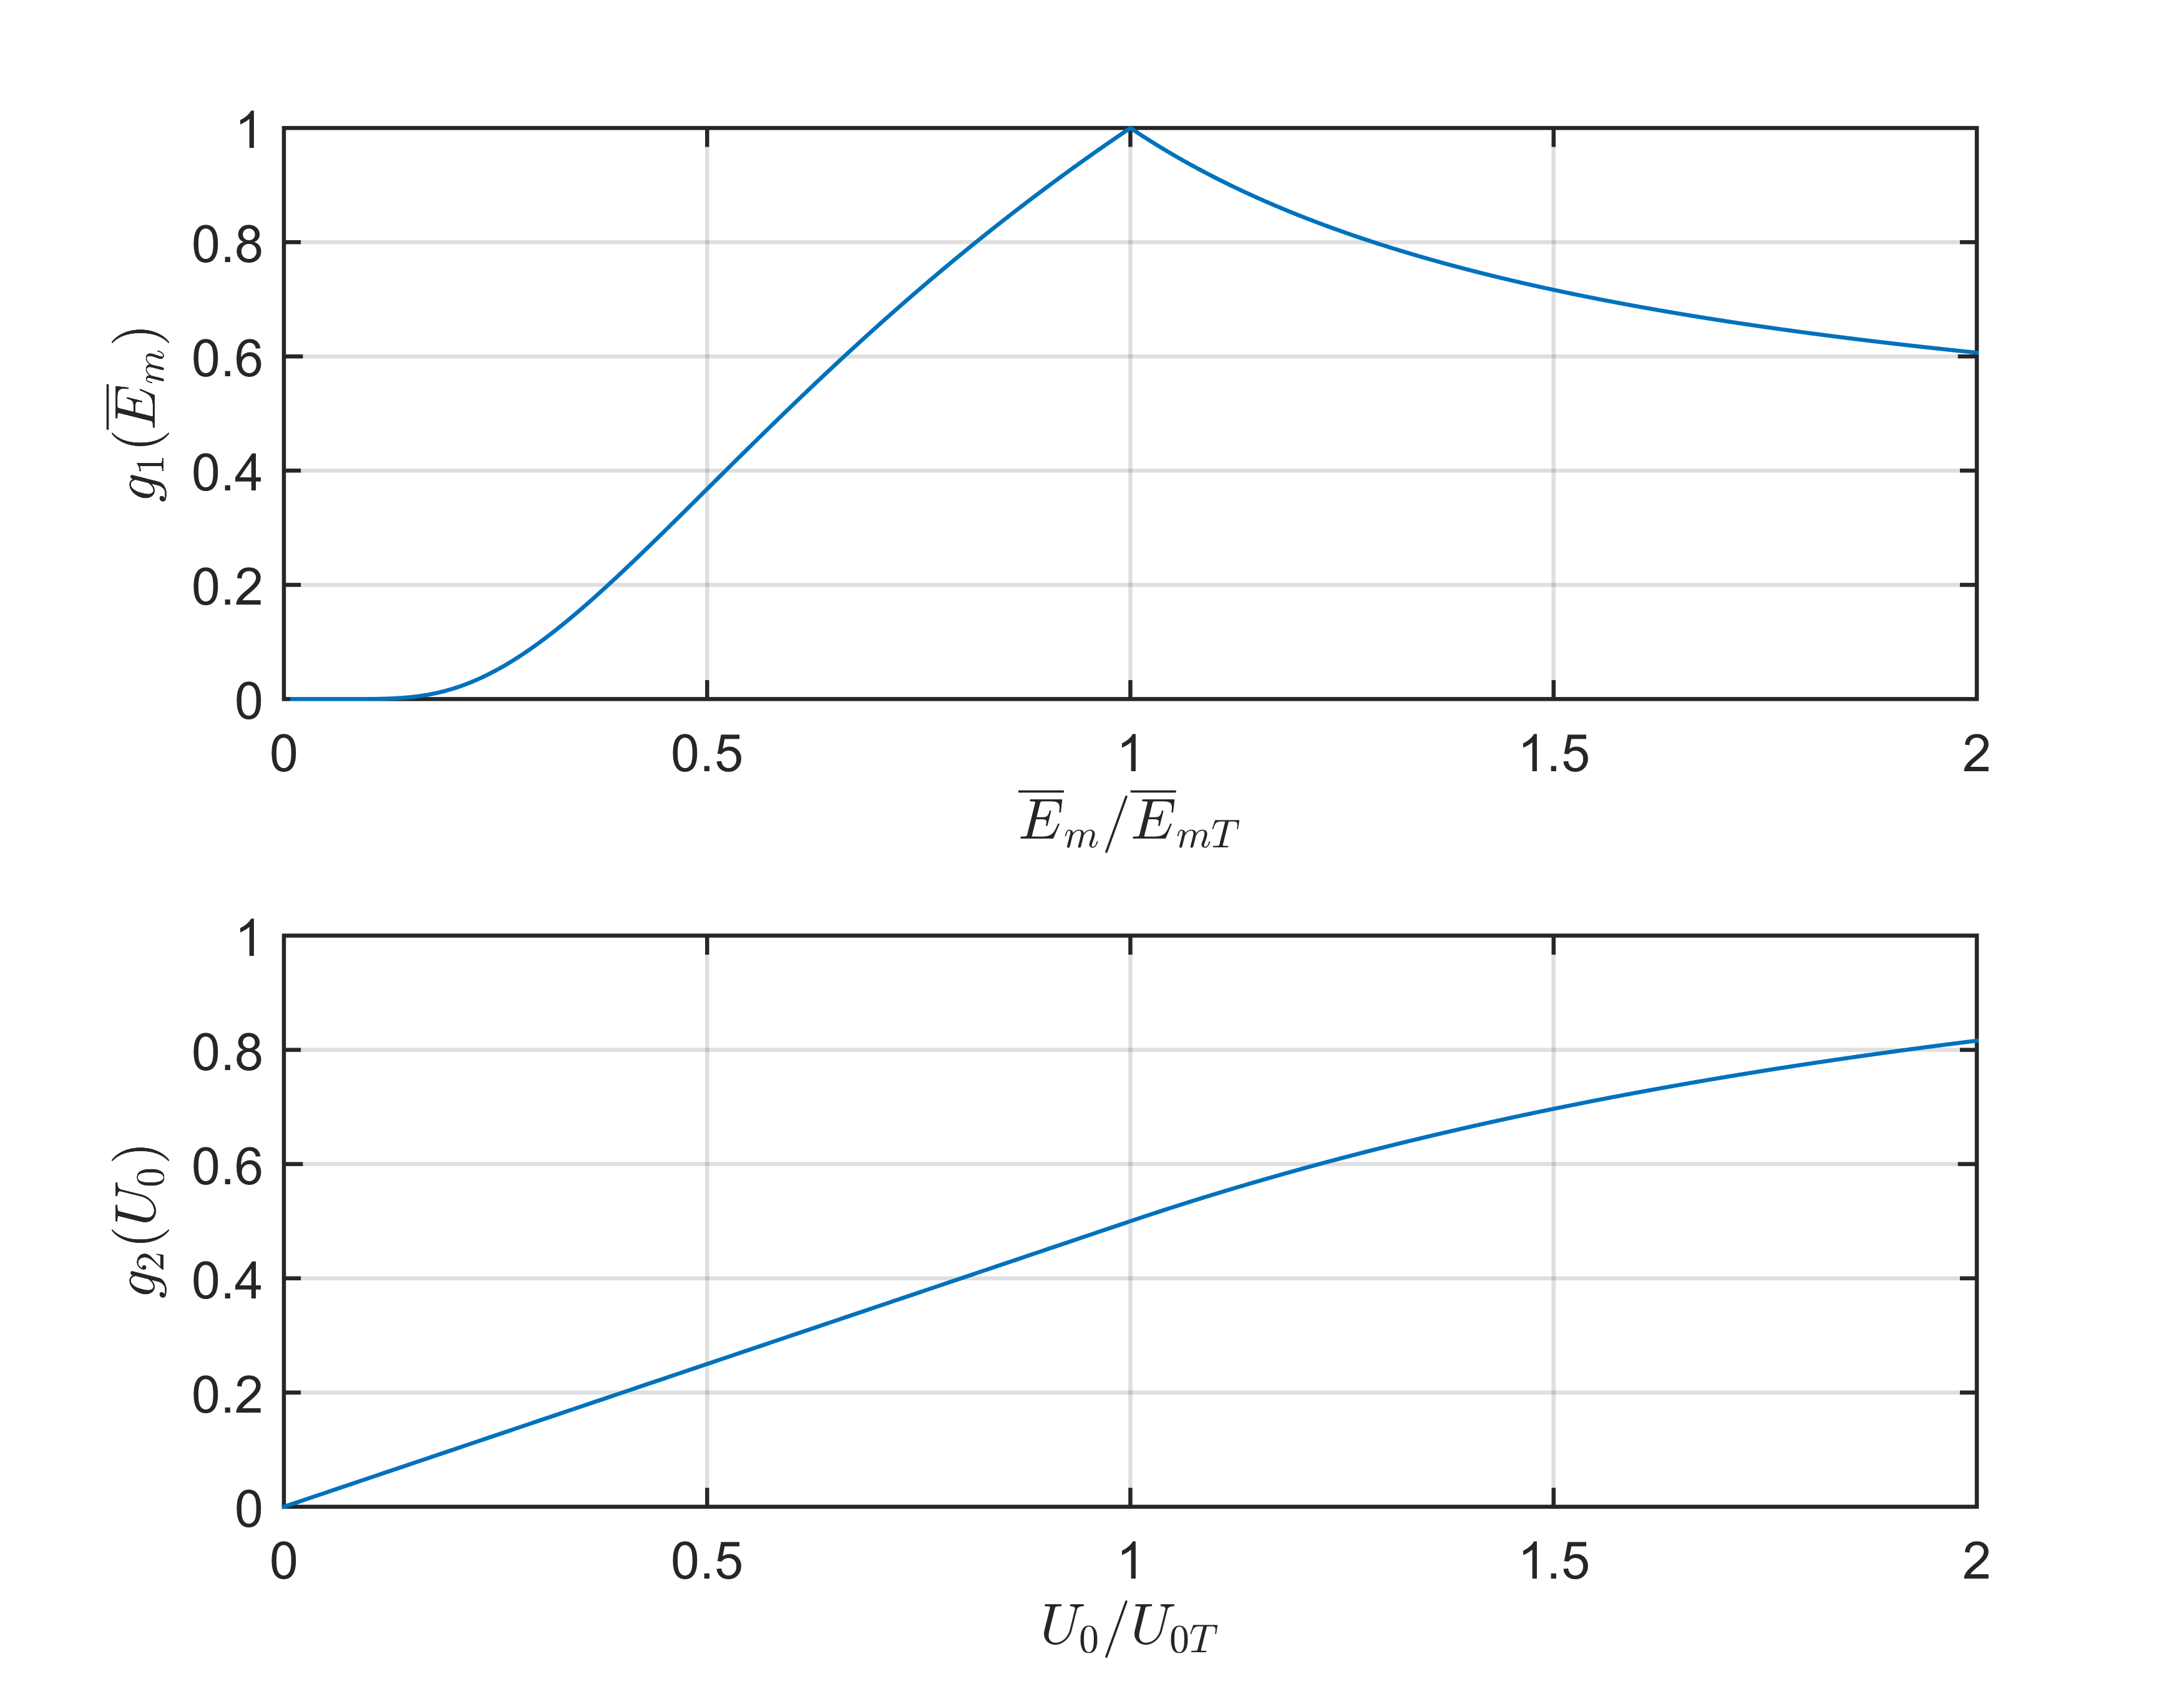
\includegraphics[width=\columnwidth]{obrG1G2}
  \caption{Graphs of parts $g_1\left(\overline{E}_{m}\right)$ and $g_2\left(U_0\right)$ from the fitness function}
  \label{fig:fitG1G2}
\end{figure}